\documentclass[aspectratio=169]{beamer}
\usepackage{graphicx}
\usepackage{listings}
\usepackage{hyperref}
\usetheme{metropolis}
\title{git/GitHub for Developers}
\institute{Engineers for Exploration, UC San Diego}
\setbeamertemplate{caption}[numbered]
\lstset{
    basicstyle=\ttfamily
}
\logo{
\includegraphics[height=.65cm,keepaspectratio]{e4e_logo_350x136.png}}
\begin{document}
\maketitle
\begin{frame}{Introduction}
    \begin{itemize}
        \item \textbf{Git} is a distributed version control system. \textbf{GitHub} is a platform for hosting Git repositories and facilitating collaboration.
        \item git/GitHub enables efficient project management and team collaboration with its version control management and branches.
        \item \textbf{Basic Commands:}
        \begin{itemize}
            \item \textit{git init}: Initialize a new Git repository.
            \item \textit{git clone}: Copy an existing repository.
            \item \textit{git add}: Stage changes for commit.
            \item \textit{git commit}: Save staged changes along with a commit message.
            \item \textit{git push}: Upload local repository content to a remote repository.
            \item \textit{git pull}: Fetch and integrate changes from a remote repository to your current branch.
            \item \textit{git branch}: List, create, or delete branches.
            \item \textit{git checkout}: Switch branches or restore working tree files.
            \item \textit{git merge}: Combine changes from different branches into your current branch.
        \end{itemize}
    \end{itemize}
\end{frame}
\begin{frame}{Git Workflows}
\begin{itemize}
    \item \textbf{Feature Branch Workflow}:
    \begin{itemize}
        \item \textbf{Description:} Each new feature is developed in its own branch to avoid disrupting the main codebase. Merging is done via pull requests to facilitate code review.
        \item \textbf{Benefits:} Keeps the main branch stable. Encourages collaboration and review before integration.
        \item \textbf{Use Case:} Ideal for ongoing projects with multiple team members working on different features simultaneously.
    \end{itemize}
    \item \textbf{Gitflow Workflow}
    \begin{itemize}
        \item \textbf{Description:} A branching model for project release management with separate branches for development, features, releases, hotfixes, and the main branch.
        \item \textbf{Benefits:} Manages releases systematically, assigns clear roles to each branch, and tracks progress more efficiently.
        \item \textbf{Use Cases:} Suited for projects with scheduled release cycles and the need for parallel releases.
    \end{itemize}
    \item \textbf{Fork Workflow}
\end{itemize}
\end{frame}
\begin{frame}{Git Workflows Cont.}
\begin{center}
    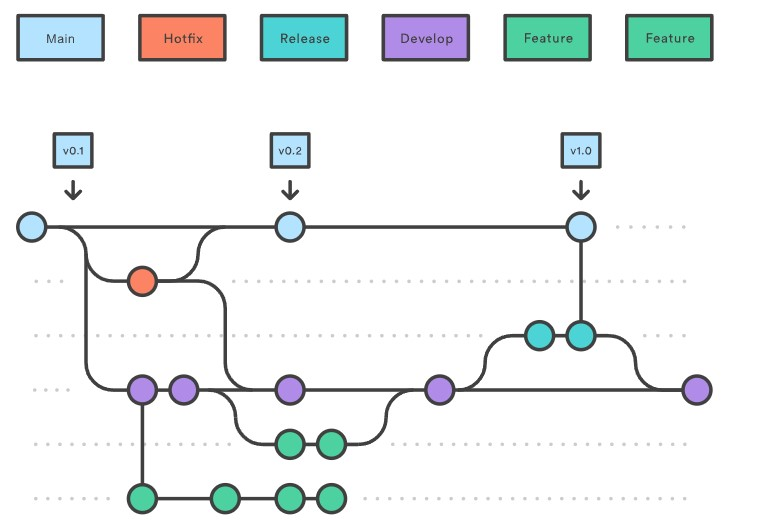
\includegraphics[scale=.6]{gitflow_workflow.jpg}
\end{center}
\end{frame}
\begin{frame}{Tags}
\begin{itemize}
    \item \textbf{Purpose of Tags:}
    \begin{itemize}
        \item Mark significant points of the project's history.
        \item Useful for marking release points (remember semantic versioning).
    \end{itemize}
    \item \textbf{Creating Tags:}
    \begin{itemize}
        \item Lightweight tags: \textit{git tag tagname}
        \item Annotated tags: \textit{git tag -a tagname -m "message"}
    \end{itemize}
    \item \textbf{Listing and Deleting Tags:}
    \begin{itemize}
        \item List all tags: \textit{git tag}
        \item Delete a tag: \textit{git tag -d tagname}
    \end{itemize}
\end{itemize}
\end{frame}
\begin{frame}{Releases}
\begin{itemize}
    \item \textbf{Creating Releases in GitHub:}
    \begin{itemize}
        \item Navigate to your repository's releases section.
        \item Draft a new release and choose the git tag that marks the version.
        \item Add release notes to describe the changes or improvements.
    \end{itemize}
    \item \textbf{Benefits of GitHub Releases:}
    \begin{itemize}
        \item Bundle source code, executable files, and other assets in one package.
        \item Provide detailed release notes to inform users about the changes or new features.
        \item Auto updates (Demo).
    \end{itemize}
\end{itemize}
\end{frame}
\begin{frame}{Pull Requests (PR) Management}
\begin{itemize}
    \item \textbf{Keep PRs Small and Focused:} Encourage contributions that are easy to review and discuss. Smaller changes are easier to understand and less likely to introduce errors.
    \item \textbf{Use a Checklist:} Develop a review checklist to ensure consistency and thoroughness. This can include code style, testing, documentation, and performance considerations.
    \item \textbf{Automated Checks:} Utilize GitHub Actions to run automated tests, linting, and other checks when PRs are opened or updated.
\end{itemize}
\end{frame}
\begin{frame}{GitHub Actions for Automation}
\begin{itemize}
    \item \textbf{Event-Driven:} Trigger workflows on GitHub events like push, pull requests, or issue comments.
    \item \textbf{Workflows and Actions:} Combine multiple actions to create workflows defined in YAML files.
    \item \textbf{Hosted Runners:} Run workflows on GitHub-hosted runners or self-hosted runners.
    \item \textbf{Examples:}
    \begin{itemize}
        \item \textbf{Automating Testing and Deployment}: Automatically run tests on every pull request or push to a specific branch. Deploy your application when a pull request is merged into the main branch.
        \item \textbf{Custom Workflows for Project Management:} Auto-assign project issues to members based on labels. Auto-label pull requests based on modified file paths.
    \end{itemize}
\end{itemize}
\end{frame}
\begin{frame}{Securing Your Project}
\begin{itemize}
    \item \textbf{Branch Protection Rules:} Configure rules to protect branches, requiring pull request reviews, status checks before merging, and more.
    \item \textbf{Dependabot:} Automatically scans your dependencies for known vulnerabilities and suggests updates or patches.
    \item \textbf{Secret Scanning:} Detects secrets and credentials exposed in your code and provides alerts.
    \item \textbf{Code Scanning:} Automatically scans your code for vulnerabilities when you push code to GitHub.
\end{itemize}
\end{frame}
\begin{frame}{Extras}
\begin{itemize}
    \item \textbf{Interactive Rebase:}
    \begin{itemize}
        \item \textbf{Definition:} Tool for rewriting history, used to edit, delete, or squash commits.
        \item \textbf{Use Case:} Cleaning up a feature branch before merging it into the main branch.
    \end{itemize}
    \item \textbf{Cherry-picking:}
    \begin{itemize}
        \item \textbf{Definition:} Allows you to pick a commit from one branch and apply it to another.
        \item \textbf{Use Case:} Applying a bug fix from one branch to another without merging all changes. 
    \end{itemize}
    \item \textbf{Stashing Changes:}
    \begin{itemize}
        \item \textbf{Definition:} Temporarily, shelves (or stashes) change so you can work on a different task.
        \item \textbf{Use Case:} Switching between branches without committing half-done work.
    \end{itemize}
\end{itemize}
\end{frame}
\end{document}